\documentclass[a4paper,12pt]{article}
\makeatletter
\renewcommand{\@seccntformat}[1]{}
\makeatother
%%% Работа с русским языком			% поиск в PDF
\usepackage{mathtext} 				% русские буквы в формулах
\usepackage[T2A]{fontenc}			% кодировка
\usepackage[utf8]{inputenc}			% кодировка исходного текста
\usepackage[english, russian]{babel}	% локализация и переносы
\usepackage{indentfirst}
\frenchspacing
\usepackage{lscape}
%%% Дополнительная работа с математикой
\usepackage{amsmath,amsfonts,amssymb,amsthm,mathtools} % AMS
\usepackage{icomma} % "Умная" запятая: $0,2$ --- число, $0, 2$ --- перечисление

%% Номера формул
%\mathtoolsset{showonlyrefs=true} % Показывать номера только у тех формул, на которые есть \eqref{} в тексте.
%\usepackage{leqno} % Нумерация формул слева

%% Свои команды
\DeclareMathOperator{\sgn}{\mathop{sgn}}

%% Перенос знаков в формулах (по Львовскому)
\newcommand*{\hm}[1]{#1\nobreak\discretionary{}
	{\hbox{$\mathsurround=0pt #1$}}{}}

%%% Работа с картинками
\usepackage{graphicx}  % Для вставки рисунков
\setlength\fboxsep{3pt} % Отступ рамки \fbox{} от рисунка
\setlength\fboxrule{1pt} % Толщина линий рамки \fbox{}
\usepackage{wrapfig} % Обтекание рисунков текстом

%%% Работа с таблицами
\usepackage{array,tabularx,tabulary,booktabs} % Дополнительная работа с таблицами
\usepackage{longtable}  % Длинные таблицы
\usepackage{multirow} % Слияние строк в таблице

%%% Программирование
\usepackage{etoolbox} % логические операторы

%%% Страница
\usepackage{extsizes} % Возможность сделать 14-й шрифт
\usepackage[margin=1in]{geometry} % Простой способ задавать поля
\geometry{top=20mm}
\geometry{bottom=20mm}
\geometry{left=15mm}
\geometry{right=15mm}

\usepackage{fancyhdr}

\pagestyle{fancy}
\fancyhf{}
\fancyhead[L]{\slshape\nouppercase{\leftmark}}
\cfoot{\thepage}

%\usepackage{fancyhdr} % Колонтитулы
% 	\pagestyle{fancy}
%\renewcommand{\headrulewidth}{0pt}  % Толщина линейки, отчеркивающей верхний колонтитул
% 	\lfoot{Нижний левый}
% 	\rfoot{Нижний правый}
% 	\rhead{Верхний правый}
% 	\chead{Верхний в центре}
% 	\lhead{Верхний левый}
%	\cfoot{Нижний в центре} % По умолчанию здесь номер страницы

\usepackage{setspace} % Интерлиньяж
%\onehalfspacing % Интерлиньяж 1.5
%\doublespacing % Интерлиньяж 2
%\singlespacing % Интерлиньяж 1

\usepackage{lastpage} % Узнать, сколько всего страниц в документе.

\usepackage{enumitem}

\usepackage{soul} % Модификаторы начертания

\usepackage{hyperref}
\usepackage[usenames,dvipsnames,svgnames,table,rgb]{xcolor}
\hypersetup{				% Гиперссылки
	unicode=true,           % русские буквы в раздела PDF
	pdftitle={Заголовок},   % Заголовок
	pdfauthor={Автор},      % Автор
	pdfsubject={Тема},      % Тема
	pdfcreator={Создатель}, % Создатель
	pdfproducer={Производитель}, % Производитель
	pdfkeywords={keyword1} {key2} {key3}, % Ключевые слова
	colorlinks=true,       	% false: ссылки в рамках; true: цветные ссылки
	linkcolor=blue,          % внутренние ссылки
	citecolor=blue,        % на библиографию
	filecolor=magenta,      % на файлы
	urlcolor=magenta          % на URL
}

\usepackage{csquotes} % Еще инструменты для ссылок

%\usepackage[style=authoryear,maxcitenames=2,backend=biber,sorting=nty]{biblatex}

\usepackage{multicol} % Несколько колонок

\usepackage{tikz} % Работа с графикой
\usepackage{pgfplots}
\usepackage{pgfplotstable}
%\usepackage[backend=biber, bibencoding=utf8, sorting=nty, babel=other, maxcitenames=2, bibstyle=apa, style=authoryear, sortcites, sortlocale=auto]{biblatex}
\usepackage[backend=biber, bibencoding=utf8, sorting=nty, maxcitenames=2, bibstyle=apa, style=authoryear]{biblatex}

\addbibresource{bibliography.bib}
\renewcommand*{\nameyeardelim}{\addcomma\space}

\date{\today}

\setcounter{secnumdepth}{0}

\DeclareRobustCommand{\bbone}{\text{\usefont{U}{bbold}{m}{n}1}}

\DeclareMathOperator{\EX}{\mathbb{E}}% expected value

\begin{document}
	
	\begin{titlepage}
		\newpage
		
		\begin{center}
			\large{Федеральное государственное автономное образовательное учреждение высшего образования} \\
		\end{center}
		
		\begin{center}
			\large \textbf{НАЦИОНАЛЬНЫЙ ИССЛЕДОВАТЕЛЬСКИЙ УНИВЕРСИТЕТ
				«ВЫСШАЯ ШКОЛА ЭКОНОМИКИ»
			} \\
		\end{center}
		
		\vspace{1em}
		
		\begin{center}
			\Large \textbf{Факультет экономических наук} \\
		\end{center}
		\begin{center}
			\large {по направлению подготовки Экономика} \linebreak \large {образовательная программа «Экономика»}
			
		\end{center}
		
		\vspace{2em}
		
		\vspace{0.5em}
		\rule{\linewidth}{0.3mm}
		\begin{center}
			\huge \textbf{Домашнее задание №2} \\[0.4cm]
			\LARGE \textbf{В рамках курса
				«Микроэконометрика качественных данных»
}
		\end{center}
		\rule{\linewidth}{0.3mm} \\[0.4cm]
		
		\vspace{18em}
		\begin{flushright}
			\large
			\textit{Выполнил:}\\
			Максим \textsc{Пешков} \\
			\textit{Группа:}\\
			БЭК181
			% Your name
		\end{flushright}
		
		\vspace{5em}
		
		\begin{center}
			Москва, 2021
		\end{center}
		
	\end{titlepage}
	
	\newpage
	
	\tableofcontents
	
	
	\newpage
	
	\section{О данных}
	
	В данной работе  мы будем изучать, как различные факторы влияют на зарплату женщин с учетом неслучайного отбора в число занятых.

	Обозначения переменных:
	
	\begin{itemize}
		\item lfp (в работе переименовано в \underline{employment\_dummy}) - бинарная переменная, принимающая значение 1
		      если женщина работает и 0 - в противном случае (независимая переменная)
		\item \underline{wage} - почасовая зарплата женщины (независимая переменная)
		
		\vspace{0.7cm}
		
		\item hours - количество проработанных часов за год
		\item kids5 - количество детей младше 6 лет
		\item kids618 - количество несовершеннолетних детей
		          старше пяти лет
		\item age - возраст женщины
		
		\vspace{0.3cm}
		
		\item educ (в работе переименовано в \underline{education})- число лет, потраченных женщиной на
		        получение образования
		
		\vspace{0.3cm}
		
		\item hushrs (в работе переименовано \underline{husband\_work\_hours}) - количество часов, проработанных мужем женщины
		
		\vspace{0.3cm}
		
		\item husage - возраст мужа женщины
		\item huseduc - число лет, потраченных мужем женщины на
		           получение образования
		\item huswage - зарплата мужа женщины
		\item faminc - доход семьи женщины
		\item mtr - налоговая нагрузка на женщину
		\item fatheduc - число лет, потраченных отцом женщины на
		          получение образования
		\item motheduc - число лет, потраченных матерью женщины на
		            получение образования
		            
		\vspace{0.3cm}
		
		\item unem (в работе переименовано в \underline{unemployment\_region}) - безработица в регионе проживания женщины
		
		\vspace{0.3cm}
		
		\item city - бинарная переменная, принимающая значение 1
		       если женщина живет в городе и 0 - иначе
		       
		 \vspace{0.3cm}
		 
		\item exper (в работе переименовано \underline{experience}) - рабочий стаж женщины в годах
		
	    \vspace{0.3cm}
	    
		\item nwifeinc - доход семьи женщины за вычетом ее дохода
		\item wifecoll - бинарная переменная, принимающая значение 1
		            если женщина посещала колледж и 0 - иначе
		\item huscoll - бинарная переменная, принимающая значение 1
		           если муж женщины посещал колледж и 0 - иначе
	\end{itemize}
	
	\newpage
	\section{Часть 1. Теория и гипотезы}
	
	\subsection{Задание №1.1.}
	\textit{
	Выберите независимые переменные для уравнения зарплаты и уравнения занятости. Кратко теоретически обоснуйте выбор каждой из них: не обязательно со ссылками на литературу, достаточно здравого смысла. Укажите и кратко обоснуйте предполагаемые направления эффектов. Уравнение занятости должно включать по крайней мере одну переменную, которой не было в уравнении зарплаты, и одну переменную,
	которая есть в уравнении зарплаты. Желательно, чтобы общая для двух уравнений
	переменная была непрерывной, например, возраст, а также не использовать более трех
	переменных в каждом из уравнений.}
	
	\vspace{0.3cm}
	
	Для уравнения зарплаты и зависимой переменной \textbf{wage} будем использовать следующие независимые переменные:
	
	\begin{itemize}
		\item husband\_work\_hours
		
		Количество часов, проработанных мужем, отражает несколько вещей: работает ли муж, как усердно работает, сколько может примерно зарабатывать (если считать, что все примерно одинаково зарабатывают, то можно примерно оценить среднюю возможную зарплату). Таким образом, учитывая, что для проживания семьям достаточно получать определенный средний доход, эти факторы позволяют оценить должна ли работать жена (если муж недостаточно работает или не работает вовсе), и если нужно работать, то с какими усилиями нужно, чтобы обеспечить семью достаточным для счастливого проживания общим доходом. То есть если муж мало работает, то им может не хватать денег, поэтому жена будет занимать высокооплачиваемую должность. И наоборот, если муж усердно работает, то скорей всего, у их семьи достаточный общий доход и у жены нет стимулов к усердной работе с высокой зарплатой, что также подкрепляется домашними заботами в семье, которые перекладываются на жену, ведь муж много работает.
		
		
		Следовательно, будем предполагать, что количество часов, проработанных мужем, негативно влияет на зарплату жены.
		
		\item education
	
		Существует множество исследований, показывающих, что более высокое образование положительно влияет на уровень зарплаты, так как работник обладает большим количеством знаний и навыков (более высокий человеческий капитал), что ценят на более оплачиваемых должностях и в более крупных компаниях. При этом для женщин этот эффект скорей всего более выраженный, так как в силу естественных обстоятельств (рождение детей)  многие теряют 2-3 года на получение более высокого уровня образования, поэтому разница в уровне образования у девушек более выраженная, аналогично и в уровне зарплаты наблюдается более выраженный разрыв.
		
		Следовательно, будем предполагать, что количество лет, потраченных женщиной на
		получение образования положительно влияет на зарплату жены.
		
		\item experience
		
		Аналогично уровню образования рабочий стаж женщины в годах может отображать как много знаний и умений работница получила во время работы, ведь в рабочее время все работники улучшают свои профессиональные навыки, получают больше знаний (увеличивают свой человеческий капитал), что способствует их более уверенному продвижению по карьерной лестнице, увеличивая себе уровень зарплаты. 
		
		Следовательно, будем предполагать, что рабочий стаж женщины в годах положительно влияет на зарплату жены.
		
	\end{itemize}

	
	
	Для уравнения занятости и зависимой переменной \textbf{employment\_dummy} будем использовать следующие независимые переменные:
	
	\begin{itemize}
		\item husband\_work\_hours
		
		Аналогично уровню зарплаты количество часов, проработанных мужем, может демонстрировать необходимость жены работать вовсе, ведь если муж много работает, то скорей всего, доход их семьи достаточно высокий и у жены нет высокий стимулов к работе, к тому же, домашние заботы и уход за детьми в таких условиях только уменьшают желание и возможность выходить на работу. Также если муж мало тратит время за работой, то скорей всего, жене необходимо будет работать, чтобы общий доход домохозяйства был достаточным для хорошего проживания. 
		
		Следовательно, будем предполагать, что количество часов, проработанных мужем, негативно влияет на вероятность занятости жены.
		
		\item kids5
		
		Маленькие дети требуют заботы, внимания и воспитания. Эти обязанности чаще всего перекладываются на жену, то есть мать детей. Поэтому при наличии маленьких детей в семье женщины вынуждены много времени тратить на воспитание детей, что ограничивает их от возможности выхода на работу. 
		
		Следовательно, будем предполагать, что количество детей младше 6 лет негативно влияет на вероятность занятости жены.
		
		\item unemployment\_region
		
		Общая обстановка в регионе также может влиять на занятость женщин. Если в регионе проживания высокая безработица, то скорей всего там наблюдается плохой инвестиционный климат и малое количество рабочих мест, что даже при наличии желании женщины работать ограничивает ее быть занятой. 
		
		Следовательно, будем предполагать, что безработица в регионе проживания женщины негативно влияет на вероятность занятости жены.
		
	\end{itemize}
	
	\newpage
	
	\section{Часть 2. Модель Тобина}
	
	\subsection{Задание №2.1.}
	\textit{Оцените Тобит модель, предварительно записав максимизируемую функцию
правдоподобия. Результат представьте в форме таблицы (можно, например, использовать
выдачу из stata, R или python).}

\vspace{0.2cm}

Тобит модель предполагает оценивание латентной переменной $wage_i^*$, исходя из которой определяется значение наблюдаемой переменной $wage_i$

\begin{equation*}
	wage_i^* =  \beta_0 + \beta_h \cdot husband\_work\_hours_i +\beta_{ed} \cdot education_i + \beta_{ex} \cdot experience_i + \varepsilon_i, \varepsilon_i \sim  N (0, \sigma^2)
\end{equation*}

\begin{equation*}
	wage_i = 
	\begin{cases}
		wage_i^*, wage_i^*  >  0 \\
		 0, wage_i^*  \leq 0
	\end{cases}
\end{equation*}

Исходя из этого, можно легко написать максимизируемую функцию правдоподобия (см. ниже). Где $\varphi$ - функция плотности стандартного нормального распределения, $\Phi$ - функция стандартного нормального распределения, $\sigma$ - оцениваемое стандартное отклонение  $wage_i$ если бы оно не было цензурированно, $\beta$ - вектор оцениваемых коэффициентов ($\beta_0, \beta_h, \beta_{ed}, \beta_{ex}$)'.

\begin{equation*}\label{eq1}
	\begin{aligned}
		\mathcal{L} = \prod_{wage_i^* > 0} \left[\frac{1}{\sigma} \varphi\left(\frac{wage_i-(\beta_0 + \beta_h \cdot husband\_work\_hours_i +\beta_{ed} \cdot education_i + \beta_{ex} \cdot experience_i )}{\sigma}\right) \right] \times \\ 
		\prod_{wage_i^* \leq 0} \left[1-\Phi\left(  \frac{\beta_0 + \beta_h \cdot husband\_work\_hours_i +\beta_{ed} \cdot education_i + \beta_{ex} \cdot experience_i }{\sigma}  \right)    \right] \rightarrow \max_{\beta, \sigma}
	\end{aligned}
\end{equation*}

\vspace{0.2cm}

Результат оценивания представлен на Рисунке \ref{tobit}.

\begin{figure}[!h] \centering
	\caption{Результат оценивания Тобит модели в R}
	\label{tobit}
	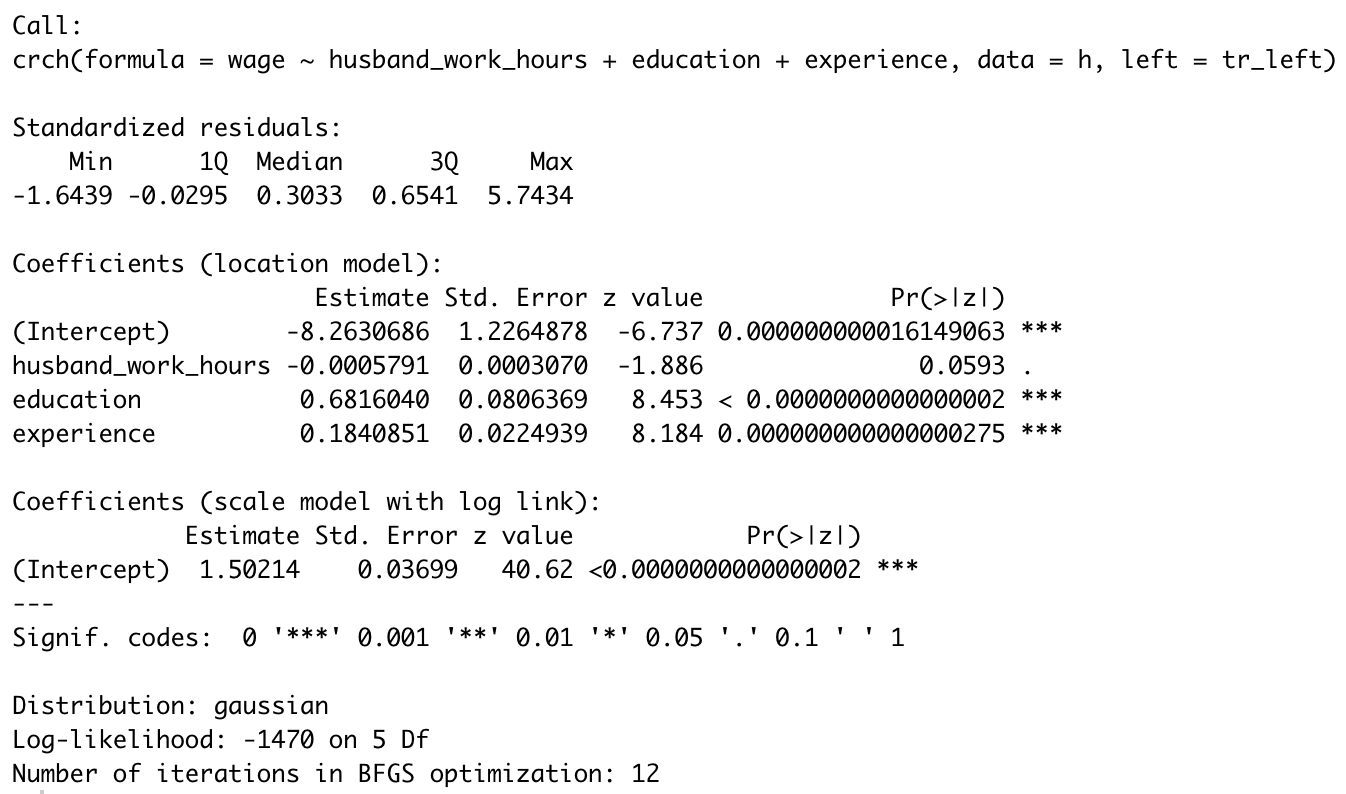
\includegraphics[scale=0.7]{tobit1.png}
\end{figure}

Из представленной выгрузки из R можно видеть, значения коэффициентов каждой переменной, их стандартные ошибки, z-статистики для проверки гипотезы о значимости коэффицентов (нулевая гипотеза заключается в равенстве коэффициента нулю) и соответствующие p-value. Также можно видеть, что коэффициенты посчитаны благодаря численной оптимизации функции правдоподобия, записанной выше, где 5 - число оцениваемых параметров (4 коэффициента $\beta$ и стандартное отклонение)

\subsection{Задание №2.2.}
\textit{Опишите преимущества Тобит модели над усеченной регрессией. Объясните, в
каких случаях можно использовать усеченную регрессию, но не получится использовать
Тобит модель: приведите гипотетический (можно использовать фантазию) пример.}

\vspace{0.2cm}

Преимущества Тобит модели над усеченной регрессией:

\begin{itemize}
	\item  Асимптотическая нормальность ошибок
	
	\item Асимптотическая состоятельность оценок 
	
	\item Более эффективные оценки 
	
	\item Не исчезают наблюдения, что позволяет оценить направленность эффекта на полной выборке и не нарушает предпосылку ТГМ
	
\end{itemize}

Усеченную регрессию можно использовать, если цензурированные наблюдения несли неважную информацию и их добавление в модели Тобина, на самом деле, будет вести к не самым эффективным оценкам. То есть в таких случаях, когда усечение необходимо из поставленного вопроса и добавлять пропущенные наблюдения не нужно (они могут не позволить ответить на поставленный вопрос). 

Возможным примером может быть исследование факторов роста акций крупных компаний  - "голубых фишек". В этом случае не нужно включать мелкие компании -  цензурированные наблюдения. Действительно, для акций мелких компаний большее значение может иметь волатильность и различные другие финансовые факторы риска, которые для крупных не так важны, поэтому для анализа поставленного вопроса лучше всего подойдет усеченная модель.


\subsection{Задание №2.3.}
\textit{Проинтерпретируйте полученные значения оценок для каждой независимой
переменной. Поясните, как полученные результаты соотносятся с высказанными вами
ранее предположениями.}

\vspace{0.2cm}

По полученным коэффициентам можно оценить предельный эффект переменной на математическое ожидание латентной зависимой переменной (то есть $\dfrac{\partial \EX (wage_i^*)}{\partial x_s}=\hat{\beta_s}$), а также оценить направленность предельного эффекта на математическое ожидание зависимой переменной (то есть $\dfrac{\partial \EX (wage_i)}{\partial x_s}=\hat{\beta_s}\Phi(\frac{x_i'\beta}{\sigma}), 1\geq \Phi(\frac{x_i'\beta}{\sigma})\geq0$) . То есть эффект на зарплату для работающих женщин (для латентной переменной) будет больше по модулю, чем для всей выборки. Исходя из этого приведем интерпретацию полученных коэффициентов.

\begin{itemize}
	\item  husband\_work\_hours - количество часов проработанных мужем за год имеет отрицательный эффект на уровень зарплаты женщины - увеличение количества часов проработанных мужем на 100 часов в среднем уменьшает почасовую зарплату работающей жены на 0.05 долларов (для общей выборки так явно не можем сказать, для них только можем утверждать про отрицательный эффект).
	
	В целом это подтверждает наше предположение, ведь чем больше работает мужчина, тем меньше нужно работать женщине и зарабатывать соответственно. Хотя коэффициент значим только на 10\% уровне значимости (используется z статистика для проверки гипотезы о равенстве коэффициента нулю), что может быть обосновано тем, что мужчина может мало работать в часах, но много зарабатывать или семье оказывает поддержку государство или родители, что тоже уменьшает стимулы женщины работать и больше зарабатывать.
	
	\item education - число лет, потраченных женщиной на
	получение образования влияет положительно на почасовую заработную плату женщины - 
	увеличение числа лет образования на 1 год в среднем увеличивает почасовую зарплату работающей жены на 0.68 долларов (для общей выборки так явно не можем сказать, для них только можем утверждать про положительный эффект).
	
	Это подтверждает наше предположение о положительном эффекте, ведь большее количество лет обучения ведет к более высокому уровню человеческого капитала, что положительно влияет на заработную плату и востребованность работника. Причем коэффициент по z-статистике значим на любом разумном уровне значимости.
	
	\item experience - рабочий стаж женщины также положительно влияет на почасовую заработную плату женщины - 
	увеличение стажа на 1 год в среднем увеличивает почасовую зарплату работающей жены на 0.18 долларов (для общей выборки так явно не можем сказать, для них только можем утверждать про положительный эффект).
	
	Это подтверждает наше предположение о положительном эффекте, ведь большее число лет в стаже ведет к более высокому уровню профессиональных  навыков, что положительно влияет на заработную плату и востребованность работника. Причем коэффициент по z-статистике значим на любом разумном уровне значимости.
	
	
\end{itemize} 



\subsection{Задание №2.4.}
\textit{Для индивида с произвольными характеристиками укажите (предварительно
записав используемые для расчетов формулы):}

\begin{enumerate}[label=\Alph*)]
	\item $\EX(y^*)$
	\item $\EX(y)$
	\item \textit{Вероятности того, что индивид работает}
\end{enumerate}

\vspace{0.2cm}

Зададим характеристики рассматриваемого индивида в Таблице \ref{individ} и рассмотрим каждый пункт отдельно.


\begin{table}[!h]
	\caption{Характеристики рассматриваемого индивида}
	\label{individ}
	\centering
	\small
	\begin{tabular}{|c|c|}
		\hline
		Переменная &  Значение  \\ 
		\hline
		$husband\_work\_hours_{ind} $ &2000 \\ 
		\hline
		$education_{ind} $ &15 \\ 		
		\hline
		$experience_{ind} $ &5 \\ 	
		\hline
	\end{tabular}
\end{table}

\begin{enumerate}[label=\Alph*)]
	\item $\EX(y^*)$
	
	Из лекций знаем, что $\EX(wage_i^*) = \hat{\beta_0}+\hat{\beta_h} \cdot husband\_work\_hours_{ind}  +\hat{\beta_{ed} }\cdot education_{ind}+ \hat{\beta_{ex} }\cdot experience_{ind}$
	
	Подставляя найденные оценки и значения для индивида находим
	
	\begin{align*}
		\EX(wage_i^*) = -8.2630685960 -0.0005790926*2000+  0.6816039702*15  +0.1840850533 *5 \\= 1.723231
	\end{align*}
	
	То есть для выбранного индивида математическое ожидание почасовой заработной платы при условии работающей женщины будет равна примерно 1.72 доллара
	
	\item $\EX(y)$
	
	Из лекций знаем, что 
	\begin{align*}
	\EX(wage_i) = (\hat{\beta_0}+\hat{\beta_h} \cdot husband\_work\_hours_{ind}  +\hat{\beta_{ed} }\cdot education_{ind}+ \hat{\beta_{ex} }\cdot experience_{ind}+\hat{\sigma}\cdot \lambda_i) \times \\ \times \Phi \left(\frac{\hat{\beta_0}+\hat{\beta_h} \cdot husband\_work\_hours_{ind}  +\hat{\beta_{ed} }\cdot education_{ind}+ \hat{\beta_{ex} }\cdot experience_{ind}}{\hat{\sigma}}\right)
	\end{align*}

	Где $\lambda_i = \dfrac{\varphi\left(\frac{\hat{\beta_0}+\hat{\beta_h} \cdot husband\_work\_hours_{ind}  +\hat{\beta_{ed} }\cdot education_{ind}+ \hat{\beta_{ex} }\cdot experience_{ind}}{\hat{\sigma}}\right)}{\Phi \left(\frac{\hat{\beta_0}+\hat{\beta_h} \cdot husband\_work\_hours_{ind}  +\hat{\beta_{ed} }\cdot education_{ind}+ \hat{\beta_{ex} }\cdot experience_{ind}}{\hat{\sigma}}\right)}$
	
	Подставим найденные оценки и значения для выбранного индивида
	
	\begin{align*}
		\lambda_i  = \dfrac{\varphi\left(\frac{-8.2630685960 -0.0005790926*2000+  0.6816039702*15  +0.1840850533 *5}{4.49129}\right)}{\Phi\left(\frac{-8.2630685960 -0.0005790926*2000+  0.6816039702*15  +0.1840850533 *5}{4.49129}\right)} =\\
		=\dfrac{\varphi(0.3836828 )}{\Phi(0.3836828 )} = 0.5707363\\
	\EX(wage_i) = (-8.2630685960 -0.0005790926*2000+  \\0.6816039702*15  +0.1840850533 *5 + 4.49129*0.5707363)\\ \times\Phi(0.3836828 ) &=\\
		=2.783672
	\end{align*}
	
	То есть для выбранного индивида математическое ожидание почасовой заработной платы будет равна примерно 2.78 доллара
	
	\item \textit{Вероятности того, что индивид работает}
	
	Из лекций знаем, что 
	\begin{align*}
			P(wage_i>0) = \Phi \left(\frac{\hat{\beta_0}+\hat{\beta_h} \cdot husband\_work\_hours_{ind}  +\hat{\beta_{ed} }\cdot education_{ind}+ \hat{\beta_{ex} }\cdot experience_{ind} }{\hat{\sigma} }\right) \\= 0.6493932
	\end{align*}
	
	То есть для выбранного индивида вероятности того, что она работает будет равна примерно 0.65.
	
\end{enumerate}


\subsection{Задание №2.5.}
\textit{
Для индивида с произвольными характеристиками рассчитайте предельный
эффект любой переменной (не дамми), входящей линейно (предварительно записав
используемые для расчетов формулы) на:}

\begin{enumerate}[label=\Alph*)]
	\item $\EX(y^*)$
	\item $\EX(y)$
	\item \textit{Вероятности того, что индивид работает}
\end{enumerate}

Зададим характеристики рассматриваемого индивида в Таблице \ref{individ} и рассмотрим каждый пункт отдельно, где будем считать предельный эффект для переменной числа лет, потраченной женщиной на получение образования $education$.

\begin{enumerate}[label=\Alph*)]
	\item $\EX(y^*)$
	
	Из лекций знаем, что $\dfrac{\partial \EX (wage_i^*)}{\partial education}=\hat{\beta_{ed}} = 0.681604$
	
	То есть увеличение числа лет образования на 1 год для выбранного индивида может увеличить почасовую зарплату работающей женщины (то есть при условии что она работает) примерно на 0.68 долларов
	
	\item $\EX(y)$
	
	
	Из лекций знаем, что 
	
	$\dfrac{\partial \EX (wage_i)}{\partial education}=\hat{\beta_{ed}}\times \Phi \left(\frac{\hat{\beta_0}+\hat{\beta_h} \cdot husband\_work\_hours_{ind}  +\hat{\beta_{ed} }\times education_{ind}+ \hat{\beta_{ex} }\cdot experience_{ind}}{\hat{\sigma} }\right)  = 0.442629$
	
	То есть увеличение числа лет образования на 1 год для выбранного индивида может увеличить почасовую зарплату примерно на 0.44 доллара (рассчитывая по всей выборке вне зависимости работала или нет).
	
	\item \textit{Вероятности того, что индивид работает}
	
	Из лекций знаем, что 
	
	
	$\dfrac{\partial  P(wage_i>0)}{\partial educ}=\frac{\hat{\beta_{ed}}}{\hat{\sigma}}\times\varphi \left(\frac{\hat{\beta_0}+\hat{\beta_h} \cdot husband\_work\_hours_{ind}  +\hat{\beta_{ed} }\cdot education_{ind}+ \hat{\beta_{ex} }\cdot experience_{ind}}{\hat{\sigma} }\right)  = 0.05624763$
	
	То есть увеличение числа лет образования на 1 год для выбранного индивида может увеличить вероятность стать занятым на 5\%.
	
\end{enumerate}




\subsection{Задание №2.6.*}
\textit{Добавьте в модель нелинейный эффект (например, квадрат). Повторите
предыдущий пункт для переменной, имеющей нелинейный эффект.}

\vspace{0.2cm}


Исследуем квадратичное влияние на почасовую зарплату женщин у количества лет потраченное на получение образования. По нескольким причинам будем предполагать обнаружить перевернутую U-образную зависимость. Причинами для такого возможного наличия следующие: при большом количестве лет обучения после определенного уровня происходит переобучение женщин и их зарплата будет только уменьшаться с увеличением количества лет обучения, так как на рынке труда не нужны переквалифицированные люди с множеством навыков; также возможно женщины с большим количеством лет получения образования собираются идти в определенные профессии, которые на самом деле менее оплачиваемые (например, в науку). Поэтому новая модель  будет задано следующим уравнениями:


\begin{equation*}
	wage_i^* =  \beta_0 + \beta_h \cdot husband\_work\_hours_i +\beta_{ed} \cdot education_i + \beta_{ex} \cdot experience_i + \beta_{ed2} \cdot education_i^2 +  \varepsilon_i
\end{equation*}

\begin{equation*}
	wage_i = 
	\begin{cases}
		wage_i^*, wage_i^*  >  0 \\
		0, wage_i^*  \leq 0
	\end{cases}
\end{equation*}

Результаты оценивания такой регрессии представлены на Рисунке \ref{tobit2}


\begin{figure}[!h] \centering
	\caption{Результат оценивания Тобит модели в R с нелинейным вхождением лет образования }
	\label{tobit2}
	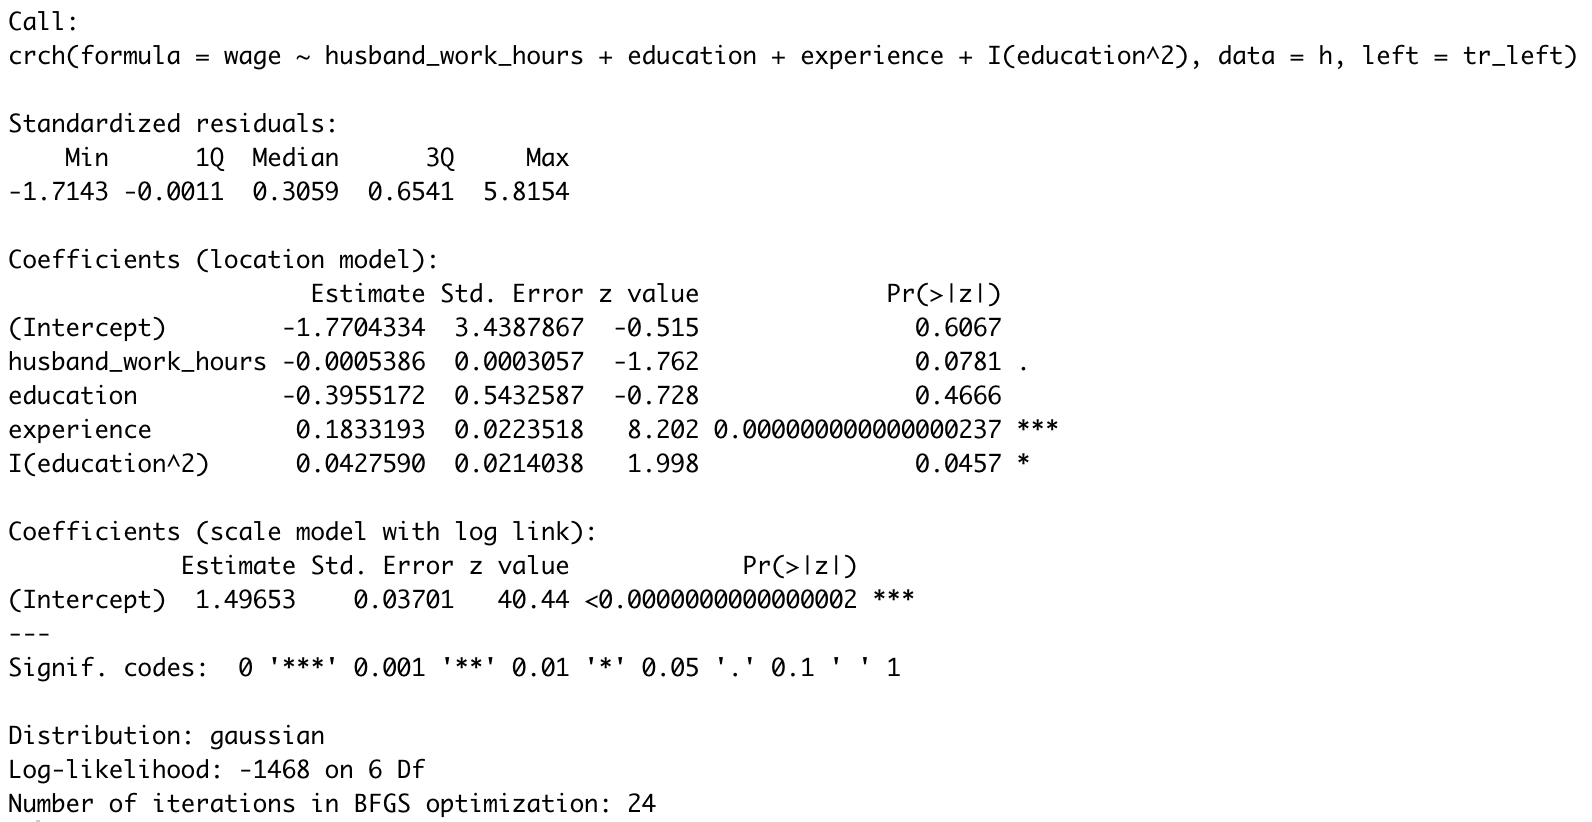
\includegraphics[scale=0.67]{tobit2.png}
\end{figure}

Из представленной выгрузки из R можно видеть, значения коэффициентов каждой переменной, их стандартные ошибки, z-статистики для проверки гипотезы о значимости коэффицентов (нулевая гипотеза заключается в равенстве коэффициента нулю) и соответствующие p-value. Также можно видеть, что коэффициенты посчитаны благодаря численной оптимизации функции правдоподобия, записанной выше, где 6 - число оцениваемых параметров (5 коэффициента $\beta$ и стандартное отклонение). Также видно, что коэффициент перед количеством часов проработанных мужем также значим только на 10\% уровне значимости, число лет рабочего стажа значим на любом разумном уровне значимости, а число лет потраченное на получение образования при линейном вхождении не значим, а при квадратичном значим на 5\% уровне значимости, что частично подтверждает наше предположение, но необходимо посчитать предельные эффекты.

Посчитаем предельные эффекты для выбранного индивида, чьи характеристики представлены в Таблице \ref{individ}.

\begin{enumerate}[label=\Alph*)]
	\item $\EX(y^*)$
	
	Из лекций знаем, что 
	
	$\EX(wage_i^*) = \hat{\beta_0} + \hat{\beta_h}\cdot husband\_work\_hours_i +\hat{\beta_{ed} }\cdot education_i + \hat{\beta_{ed2} }\cdot education_i^2 + \hat{\beta_{ex}}\cdot experience_i $
	
	Так как математическое ожидание не зависит от форм вхождения независимых переменных. Отсюда легко найдем предельный эффект:
	
	\begin{align*}
		\dfrac{\partial \EX (wage_i^*)}{\partial education}=\hat{\beta_{ed}} +2* \hat{\beta_{ed2} }*education_i = 0.8872537 
	\end{align*}
	
	То есть увеличение числа лет образования на 1 год для выбранного индивида может увеличить почасовую зарплату работающей женщины примерно на 0.88 долларов
	
	
	\item $\EX(y)$
	
	Из лекций знаем, что $E(wage_i)$ имеет такую же формулу, так как математическое ожидание не зависит от форм вхождения независимых переменных. 
	
	$
		\EX(wage_i) = (\hat{\beta_0} + \hat{\beta_h}\cdot husband\_work\_hours_i +\hat{\beta_{ed} }\cdot education_i + \hat{\beta_{ed2} }\cdot education_i^2 + \hat{\beta_{ex}}\cdot experience_i +\hat{\sigma}\cdot \lambda_i) \times \Phi \left(\frac{\hat{\beta_0} + \hat{\beta_h}\cdot husband\_work\_hours_i +\hat{\beta_{ed} }\cdot education_i + \hat{\beta_{ed2} }\cdot education_i^2 + \hat{\beta_{ex}}\cdot experience_i  }{\hat{\sigma}}\right)
	$
	
	
		Где $\lambda_i = \dfrac{\varphi\left(\frac{\hat{\beta_0} + \hat{\beta_h}\cdot husband\_work\_hours_i +\hat{\beta_{ed} }\cdot education_i + \hat{\beta_{ed2} }\cdot education_i^2 + \hat{\beta_{ex}}\cdot experience_i }{\hat{\sigma}}\right)}{\Phi \left(\frac{\hat{\beta_0} + \hat{\beta_h}\cdot husband\_work\_hours_i +\hat{\beta_{ed} }\cdot education_i + \hat{\beta_{ed2} }\cdot education_i^2 + \hat{\beta_{ex}}\cdot experience_i }{\hat{\sigma}}\right)}$
		
	Путем взятия производных и подсчета можно получить, что 
		
	$
		\dfrac{\partial \EX (wage_i)}{\partial education}=(\hat{\beta_{ed}}+2* \hat{\beta_{ed2} }*education_i)\times \\ \times\Phi \left(\frac{\hat{\beta_0} + \hat{\beta_h}\cdot husband\_work\_hours_i +\hat{\beta_{ed} }\cdot education_i + \hat{\beta_{ed2} }\cdot education_i^2 + \hat{\beta_{ex}}\cdot experience_i  }{\hat{\sigma} }\right)
		= 0.5793682 
	$

	То есть увеличение числа лет образования на 1 год для выбранного индивида может увеличить почасовую зарплату примерно на 0.58 доллара (рассчитывая по всей выборке вне зависимости работала или нет).
	
	\item \textit{Вероятности того, что индивид работает}
	
	Из лекций знаем, что 
	
	$
		P(wage_i>0) = \Phi \left(\frac{\hat{\beta_0} + \hat{\beta_h}\cdot husband\_work\_hours_i +\hat{\beta_{ed} }\cdot education_i + \hat{\beta_{ed2} }\cdot education_i^2 + \hat{\beta_{ex}}\cdot experience_i  }{\hat{\sigma} }\right)
	$
	
	Путем взятия производных и подсчета можно получить, что 
	
	\begin{align*}
			&\dfrac{\partial  P(wage_i>0)}{\partial education}=\frac{\hat{\beta_{ed}}+2* \hat{\beta_{ed2} }*education_i}{\hat{\sigma}}\times \\ &\times
			\varphi \left(\frac{\hat{\beta_0} + \hat{\beta_h}\cdot husband\_work\_hours_i +\hat{\beta_{ed} }\cdot education_i + \hat{\beta_{ed2} }\cdot education_i^2 + \hat{\beta_{ex}}\cdot experience_i }{\hat{\sigma} }\right)=\\
			&= 0.07335294 
	\end{align*}

	То есть увеличение числа лет образования на 1 год для выбранного индивида может увеличить вероятность стать занятым на 7\%.
	
	
\end{enumerate}


\subsection{Задание №2.7.**}
\textit{При помощи LR теста проверьте гипотезу о гомоскедастичности в Тобит
модели, предварительно формально записав предполагаемые нулевой гипотезой
ограничения на параметры, асимптотическое распределение тестовой статистики (при
верной нулевой гипотезе) и максимизируемую в гетероскедастичной Тобит модели
функцию правдоподобия. При этом уравнение дисперсии должно включать по крайней
мере одну переменную, не входящую в основное уравнение. Укажите негативные
последствия, к которым может приводить отсутствие учета гетероскедастичности при
условии ее наличия в Тобит модели.}


\vspace{0.2cm}

В гетероскедастичной Тобит модели будем предполагать, что дисперсия ошибки зависит от возраста (чем больше возраст, тем больше разброс в зарплатах, кто-то становится более успешным, кто-то менее успешным), а также будет зависеть от рабочего стажа (аналогично возрасту с более высоким стажем увеличивается разброс в зарплатах). Причем учитывая, что при оценивании Тобит модели находится логарифм стандартной ошибки, то будем предполагать такую зависимость $log(\sigma_i) = \gamma_0+\gamma_a*age_i+\gamma_e*experience_i+u_i$. 

В гетероскедастичной модели Тобита в функции правдоподобия будет также включена оценка параметров для ошибок, а именно 

\begin{equation*}\
	\begin{aligned}
		\mathcal{L} = \prod_{wage_i^* > 0} \left[\frac{1}{exp(\gamma_0+\gamma_a*age_i+\gamma_e*experience_i)}\times \right. \\ \left. \varphi\left(\frac{wage_i-(\beta_0 + \beta_h \cdot husband\_work\_hours_i +\beta_{ed} \cdot education_i + \beta_{ex} \cdot experience_i )}{\gamma_0+\gamma_a*age_i+\gamma_e*experience_i}\right) \right] \times \\ 
		\prod_{wage_i^* \leq 0} \left[1-\Phi\left(  \frac{\beta_0 + \beta_h \cdot husband\_work\_hours_i +\beta_{ed} \cdot education_i + \beta_{ex} \cdot experience_i }{\gamma_0+\gamma_a*age_i+\gamma_e*experience_i}  \right)    \right] \rightarrow \max_{\beta, \gamma}
	\end{aligned}
\end{equation*}

Где $\varphi$ - функция плотности стандартного нормального распределения, $\Phi$ - функция стандартного нормального распределения, $\sigma$ - оцениваемое стандартное отклонение  $wage_i$ если бы оно не было цензурированно, $\beta$ - вектор оцениваемых коэффициентов ($\beta_0, \beta_h, \beta_{ed}, \beta_{ex}$)', $\gamma$ - вектор оцениваемых коэффициентов ($\gamma_0, \gamma_a, \gamma_e$)'. То есть в этой модели оцениваемых параметров 7. 

Результаты оценивания представлены на Рисунке \ref{tobit3}.

\begin{figure}[!h] \centering
	\caption{Результат оценивания гетероскедастичной Тобит модели в R }
	\label{tobit3}
	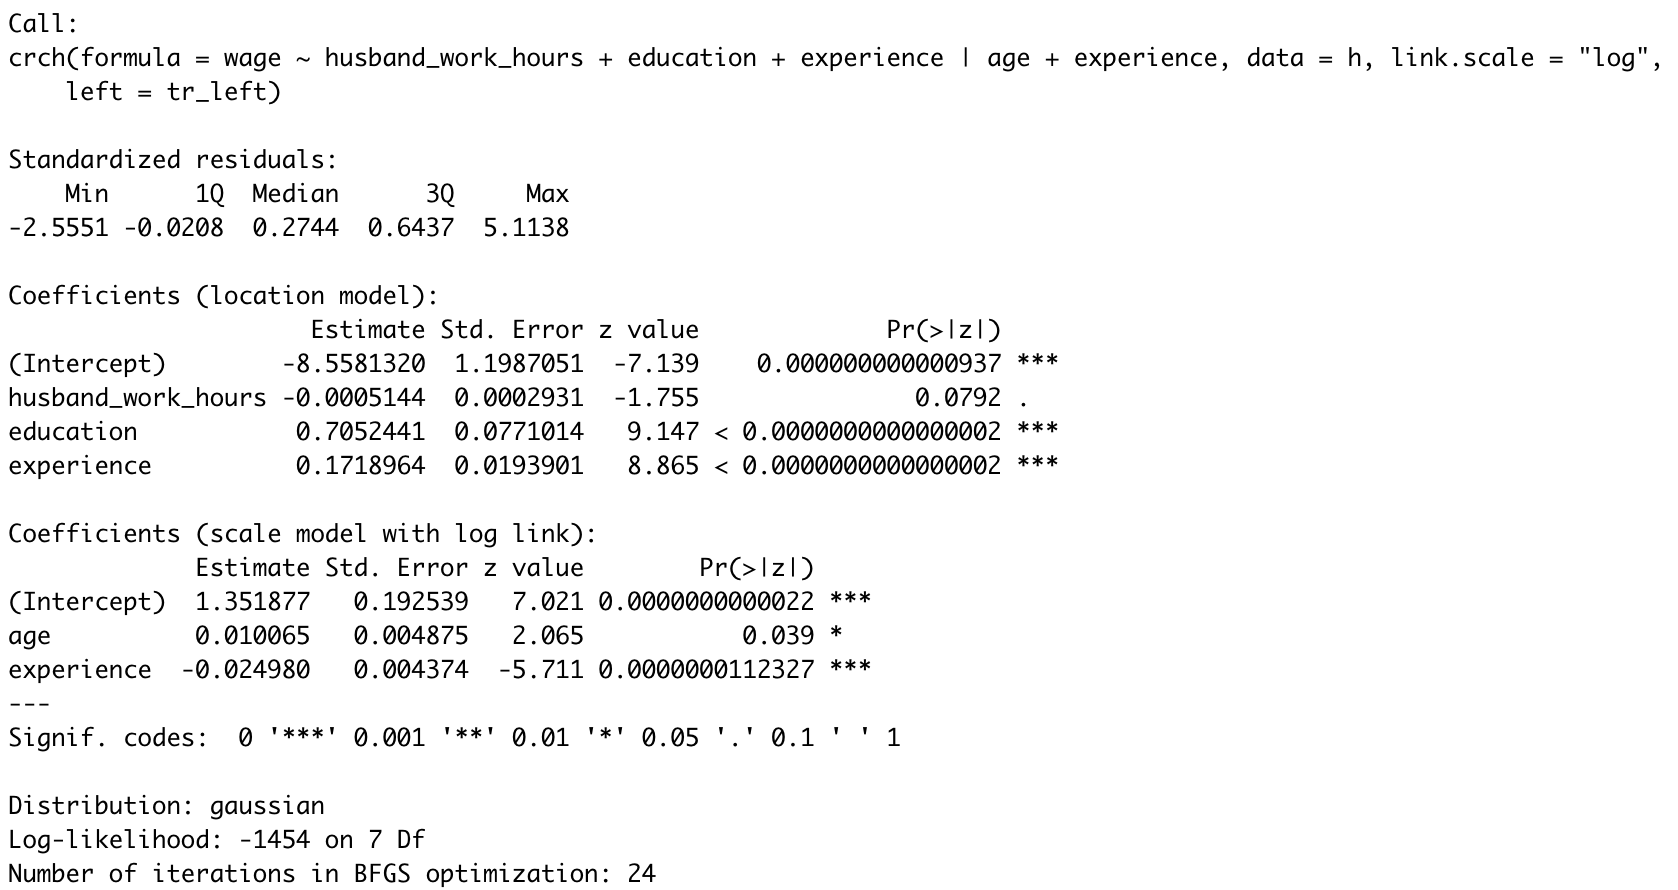
\includegraphics[scale=0.6]{tobit3.png}
\end{figure}

В LR тесте на проверку гомоскедастичности нулевая гипотеза будет заключаться в том, что $\gamma_a= \gamma_e=0$. Ограниченная модель будет модель Тобита без учета возможной гетероскедастичности, а полная модель будет модель Тобита с учетом возможной гетероскедастичности.

\begin{equation*}
	\begin{cases}
		H0: \gamma_a= \gamma_e=0\\
		Ha: \gamma_a^2+ \gamma_e^2 \ne 0
	\end{cases}
\end{equation*}

При этом как обычно тестовая статистика при верной нулевой гипотезе будет равна $2*(LR_{F} - LR_{R}) \sim \chi^2_{(m-n)}$, где LR - значения функций правдоподобий в полной и ограниченной моделях, m и n - количество параметров, оцениваемых в моделях, в нашем случае они равны 7 и 5, то есть их разница будет 2.

Таким образом получаем, что

$
LR_{statistic}=2*(LR_{F} - LR_{R})  = 2*(-1454.415 - (-1470.356)) = 31.88393 \sim\chi^2_2
$

Откуда получаем, что p-value = 0.0000001192596, то есть на лубом разумном  уровне значимости нулевая гипотеза отвергается, а значит существует гетероскедастичность в модели.

Не учет гетероскедастичности может привести к таким негативным последствиям

\begin{itemize}
	\item Неэффективность оценок
	\item Возможная потеря состоятельности оценок
	\item Искажение в оценивании предельных эффектов (особенно для тех факторов, которые еще влияют на гетероскедастичность)
\end{itemize}

\subsection{Задание №2.8.***}
\textit{
Для индивида с произвольными характеристиками в Тобит модели с
гетероскедастичной случайной ошибкой рассчитайте (предварительно записав
соответствующую формулу) предельный эффект переменной (не дамми), входящей и в
основное уравнение, и в уравнение дисперсии, на:}

\begin{enumerate}[label=\Alph*)]
	\item $\EX(y^*)$
	\item $\EX(y)$
	\item \textit{Вероятности того, что индивид работает}
\end{enumerate}


Посчитаем предельные эффект для переменной $experience$, входящей в оба уравнения по пунктам для индивида, чьи характеристики представлены в Таблице \ref{individhet}

\begin{table}[!h]
	\caption{Характеристики рассматриваемого индивида}
	\label{individhet}
	\centering
	\small
	\begin{tabular}{|c|c|}
		\hline
		Переменная &  Значение  \\ 
		\hline
		$husband\_work\_hours_{ind} $ &2000 \\ 
		\hline
		$education_{ind} $ &15 \\ 		
		\hline
		$experience_{ind} $ &5 \\ 	
		\hline
		$age_{ind} $ &45 \\ 	
		\hline
	\end{tabular}
\end{table}

\begin{enumerate}[label=\Alph*)]
	
	\item $\EX(y^*)$
	
	Так как в гетероскедастичной модели Тобита математическое ожидание не изменяется и является просто линейным индексом с оцененными параметрами $\beta$, то и предельный эффект тоже будет равен коэффициенту $\hat{\beta_{ex}}$.
	
	Таким образом
	
	\begin{align*}
		\dfrac{\partial \EX (wage_i^*)}{\partial experience}=\hat{\beta_{ex}}  = 0.1718964
	\end{align*}
	
	То есть увеличение числа лет рабочего стажа на 1 год для выбранного индивида может увеличить почасовую зарплату работающей женщины примерно на 0.17 долларов

	
	\item $\EX(y)$
	
	Зная из лекций, что 
	$\EX(wage_i) = x_i'\hat{\beta}*\Phi(\frac{x_i'\hat{\beta}}{\hat{\sigma}}) + \hat{\sigma}*\varphi(\frac{x_i'\hat{\beta}}{\hat{\sigma}}) = x_i'\hat{\beta}*\Phi(\frac{x_i'\hat{\beta}}{exp(z_i'\hat{\gamma})}) + exp(z_i'\hat{\gamma})*\varphi(\frac{x_i'\hat{\beta}}{exp(z_i'\hat{\gamma})})$
	
	Где  $\Phi$ - функция распределения у стандартного нормального распределения, $\varphi$ - функция плотности стандартного нормального распределения, 
	$\hat{\beta}$ - вектор оцененных коэффициентов ($\hat{\beta_0}, \hat{\beta_h}, \hat{\beta_{ed}}, \hat{\beta_{ex}}$)', $x_i'$  -  вектор значений переменных (1, $husband\_work\_hours_i$, $education_i$, $experience_i$),
	$\hat{\gamma}$ - вектор оцененных коэффициентов ($\hat{\gamma_0}, \hat{\gamma_a}, \hat{\gamma_e}$)',
	$z_i$'  -  вектор значений переменных в уравнении дисперсии (1, $age_i$, $experience_i$).  
	
	 То путем взятия производных и вычислений нетрудно получить, что
	 
	 $\dfrac{\partial \EX (wage_i)}{\partial experience}=\hat{\beta_{ed}}\times \Phi \left(\frac{\hat{\beta_0}+\hat{\beta_h} \cdot husband\_work\_hours_{ind}  +\hat{\beta_{ed} }\times education_{ind}+ \hat{\beta_{ex} }\cdot experience_{ind}}{\hat{\sigma} }\right) + \gamma_e*\hat{\sigma}*\varphi\left(\frac{\hat{\beta_0}+\hat{\beta_h} \cdot husband\_work\_hours_{ind}  +\hat{\beta_{ed} }\times education_{ind}+ \hat{\beta_{ex} }\cdot experience_{ind}}{\hat{\sigma} }\right) = 0.05877214$
	
	То есть увеличение числа лет стажа на 1 год для выбранного индивида может увеличить почасовую зарплату примерно на 0.06 доллара (рассчитывая по всей выборке вне зависимости работала или нет).
	
	\item \textit{Вероятности того, что индивид работает}
	
	Из лекций знаем, что 
	
	\begin{align*}
		P(wage_i>0) = \Phi \left(\frac{\hat{\beta_0}+\hat{\beta_h} \cdot husband\_work\_hours_{ind}  +\hat{\beta_{ed} }\cdot education_{ind}+ \hat{\beta_{ex} }\cdot experience_{ind} }{\hat{\sigma} }\right) 
	\end{align*}
	
	
	Путем взятия производных нетрудно получить, что
	
	$
	\dfrac{\partial  P(wage_i>0)}{\partial  experience}=
	\varphi \left(\frac{\hat{\beta_0}+\hat{\beta_h} \cdot husband\_work\_hours_{ind}  +\hat{\beta_{ed} }\cdot education_{ind}+ \hat{\beta_{ex} }\cdot experience_{ind} }{\hat{\sigma} }\right) \times \\ \times
	\left(\frac{\hat{\beta_{ex}}}{\hat{\sigma}} - (\hat{\beta_0}+\hat{\beta_h} \cdot husband\_work\_hours_{ind}  +\hat{\beta_{ed} }\cdot education_{ind}+ \hat{\beta_{ex} }\cdot experience_{ind} )*\frac{\hat{\gamma_{e}}}{\hat{\sigma}}\right) = \\ = 0.01528326
	$
	
	То есть увеличение числа лет рабочего стажа на 1 год для выбранного индивида может увеличить вероятность стать занятым на 1.5\%.
	
\end{enumerate}



\newpage

\section{Часть 3. Модель Хекмана}

\subsection{Задание №3.1.}
\textit{Оцените модель Хекмана с помощью метода максимального правдоподобия,
предварительно записав максимизируемую функцию правдоподобия и указав независимые
переменные в уравнении занятости, которое должно иметь по крайней мере одну
переменную, не входящую в уравнение зарплаты. Результат представьте в форме таблицы
(можно, например, использовать выдачу из stata, R или python).
}

\vspace{0.2cm}

В модели Хекмана задаются два уравнения с отдельными латентными зависимыми переменными: уравнения участия \ref{partip} и уравнения интенсивности \ref{inten}. Причем считается, что ошибки имеют совместное нормальное распределение c коэффициентом корреляции $\rho$.

Исходя из уравнения участия (дамми на занятость) находится $employment\_dummy_i$, по которому определяется наблюдаем ли мы зарплату или нет, и какую зарплату наблюдаем. 


\begin{equation}\label{partip}
	\begin{aligned}
			employment\_dummy_i^* =\gamma_0+ \gamma_h \cdot husband\_work\_hours_i + \gamma_k \cdot kids5_i +  \gamma_u \cdot unemployment\_region_i + u_i
	\end{aligned}
\end{equation}

\begin{equation}\label{inten}
	\begin{aligned}
			wage_i^* =\beta_0+ \beta_h \cdot husband\_work\_hours_i  +\beta_{ed} \cdot education_i + \beta_{ex} \cdot experience_i + \varepsilon_i
	\end{aligned}
\end{equation}

\begin{align*}
	\begin{pmatrix}
		\varepsilon_i\\
		u_i
	\end{pmatrix} &\sim  N
	\begin{bmatrix}
		\begin{pmatrix}
			0\\
			0
		\end{pmatrix}\!,&
		\begin{pmatrix}
			\sigma^2 & \rho \sigma  \\
			\rho \sigma & 1 
		\end{pmatrix}
	\end{bmatrix}
\end{align*}



\begin{equation*}
employment\_dummy_i= 
	\begin{cases}
		1, employment\_dummy_i^*  >  0 \\
		0, employment\_dummy_i^*  \leq 0
	\end{cases}
\end{equation*}

\begin{equation*}
	wage_i= 
	\begin{cases}
		wage_i^*, 	employment\_dummy_i = 1 \\
		\text{не  наблюдаем}, employment\_dummy_i = 0
	\end{cases}
\end{equation*}

Данную модель можно оценить методом максимального правдоподобия, разделив функции правдоподобия для тех, кто устроен на работу, и для тех кто не работает. Для работающих женщин функция правдоподобия будет строится на основе двух уравнений (используя совместное нормальное распределение ошибок), а для неработающих только на основе уравнения участия. То есть максимизируемая функция правдоподобия будет равна \ref{eq2}.

Оцениваемыми параметрами являются векторы коэффициентов $\beta, \gamma$ из уравнений \ref{inten}, \ref{partip}, а также дисперсия ошибок $\varepsilon_i$ равная $\sigma$,  а также коэффициент корреляции между ошибками уравнений ( в уравнении  $x_i$'  -  вектор значений переменных (1, $husband\_work\_hours_i$, $education_i$, $experience_i$), $z_i$-  вектор значений переменных (1, $husband\_work\_hours_i$, $kids5_i$, $unemployment\_region_i$).

\begin{equation}\label{eq2}
	\begin{aligned}
		\mathcal{L} = \prod_{employment\_dummy_i = 1} \left\{
			\left[\frac{1}{\sigma} \varphi\left(\frac{wage_i-(x_i'*\beta)}{\sigma}\right)
			\right] \times 
		\left[1  - \Phi\left(\frac{-(z_i'\gamma+\rho \cdot \frac{wage_i-(x_i'*\beta )}{\sigma})}{\sqrt{1-\rho^2}}
		\right)
		\right]
		\right\}	 \times 
		\\
	\prod_{employment\_dummy_i = 0} (1 - \Phi(z_i'\gamma ))
	 \rightarrow \max_{\beta, \gamma, \sigma, \rho}
	\end{aligned}
\end{equation}



Результаты оценивания такой регрессии представлены на Рисунке \ref{hekman1}.


\begin{figure}[!h] \centering
	\caption{Результат оценивания модели Хекмана в R, основанный на ММП}
	\label{hekman1}
	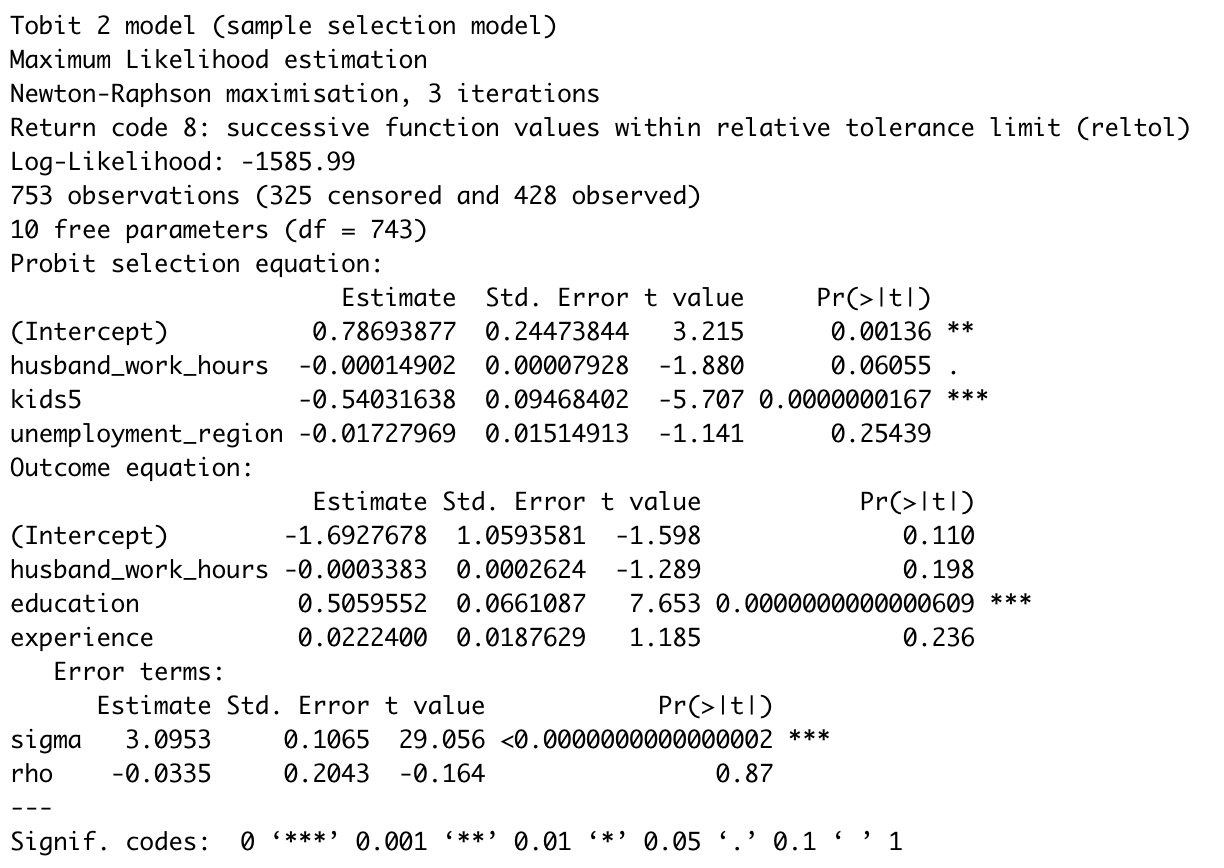
\includegraphics[scale=0.7]{heckman1.png}
\end{figure}

Из представленной выгрузки из R можно видеть, значения коэффициентов каждой переменной в каждом из 2 уравнений, их стандартные ошибки,  t-статистики для проверки гипотезы о значимости коэффициентов (нулевая гипотеза заключается в равенстве коэффициента нулю) и соответствующие p-value, также оценены $\sigma = 3.09, \rho = -0.0335$ и их тестовые статистики, по которым понятно, что коэффициент корреляции не значим. . Более того, можно видеть, что коэффициенты посчитаны благодаря численной оптимизации функции правдоподобия, записанной выше. Можно заметить и число наблюдений - 753 женщины, из которых 325 не работают и цензурированы. 


Относительно изложенных предположений о направленности эффектов в каждом из уравнений, то все коэффициенты соответствуют предположениям (они же отображают направленность предельных эффектов на латентные переменные), но малая их часть значима в каждом из уравнений. В уравнении участия значимы $husband\_work\_hours$ - на 10\% уровне значимости, а kids5 на любом разумном уровне значимости. В уравнении интенсивности значимо только количество лет для получения образования на любом разумном уровне значимости.


\subsection{Задание №3.2.} 
\textit{Опишите отличия модели Хекмана от модели Тобина.}

\vspace{0.2cm}

Можно назвать следующие отличия модели Хекмана от модели Тобина:

\begin{itemize}
	\item Не включение цензурированных наблюдений при оценивании главного уравнения, что позволяет уйти от возможных аутлаеров около нуля в модели Тобина (да и в целом в модели Хекмана логика оценивания более верная, так как в ней в основном уравнении не учитываются те, которые не прошли уравнение участие)
	
	\item Отдельный учет условия участия в другом уравнении, а не совместно, что позволяет более верно оценить эффекты по выборке (может быть так, что факторы влияют на интенсивность при участии положительно, а при участии нейтрально или отрицательно)
	
	\item Возможность оценивания других факторов на принятие решения о участии, которые могут не влиять на интенсивность, что позволяет более полно оценивать вероятность участия
	
\end{itemize}


\subsection{Задание №3.3.} 
\textit{Воспользуйтесь методом Хекмана, основанным на двухшаговой процедуре и
сравните оценки, с полученными с использованием метода Хекмана, основанном на методе
максимального правдоподобия. Опишите относительные преимущества и недостатки
обоих методов.}

\vspace{0.2cm}

Двухшаговая процедура метода Хекмана предполагает на первом шаге оценивания уравнения участия по пробит-модели, из которого находим коэффициенты $\gamma$, а также считаем $\lambda_i$ по формуле аналогичной в модели Тобина, а на втором шаге благодаря МНК находим коэффициенты $\beta$ в уравнении участия с учетом $\lambda_i$. То есть для выбранных переменных схематично можно записать так:

\begin{enumerate}
	\item Probit 
	
	\begin{equation*}
		\begin{aligned}
			P(employment\_dummy_i=1) =\gamma_0+ \gamma_h \cdot husband\_work\_hours_i + \gamma_k \cdot kids5_i +  \\ + \gamma_u \cdot unemployment\_region_i + u_i
		\end{aligned}
	\end{equation*}

Отсюда находим оценки для $\gamma_h, \gamma_k, \gamma_u$, а также

$\hat{\lambda_i }= \dfrac{\varphi(\hat{\gamma_0}+ \hat{\gamma_h} \cdot husband\_work\_hours_i  + \hat{\gamma_k} \cdot kids5_i +  \hat{\gamma_u} \cdot unemployment\_region_i   )}{\Phi (\hat{\gamma_0}+  \hat{\gamma_h} \cdot husband\_work\_hours_i  + \hat{\gamma_k} \cdot kids5_i +  \hat{\gamma_u} \cdot unemployment\_region_i  )}$

\item МНК

\begin{equation*}
	\begin{aligned}
		wage_i = \beta_h \cdot husband\_work\_hours_i  +\beta_{ed} \cdot education_i + \beta_{ex} \cdot experience_i + \beta_{\lambda}\cdot\hat{\lambda_i }+  \varepsilon_i
	\end{aligned}
\end{equation*}

Отсюда находим оценки для $\beta_h, \beta_{ed}, \beta{ex}$
\end{enumerate}

Результаты оценивания методом Хекмана по двухшаговой процедуре представлены на Рисунке \ref{hekman2}.

\begin{figure}[!h] \centering
	\caption{Результат оценивания модели Хекмана в R, основанный на двухшаговой процедуре}
	\label{hekman2}
	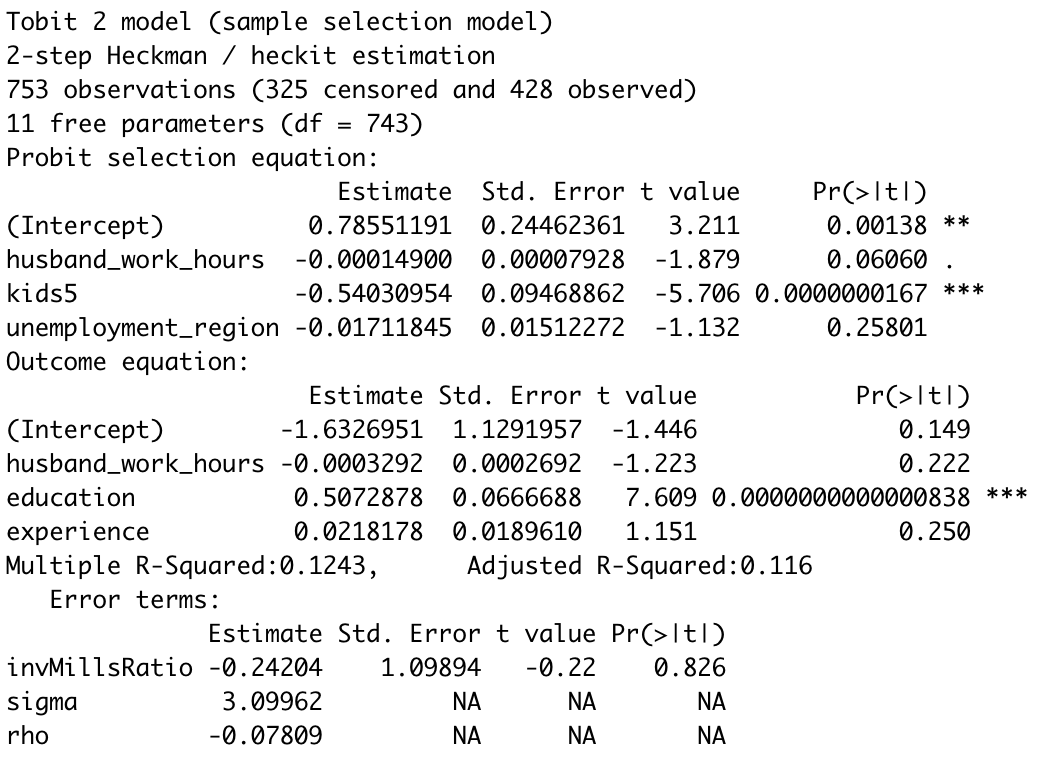
\includegraphics[scale=0.58]{heckman2step.png}
\end{figure}

 Из представленной выгрузки из R можно видеть, значения коэффициентов каждой переменной в каждом из 2 уравнений, их стандартные ошибки,  t-статистики для проверки гипотезы о значимости коэффициентов (нулевая гипотеза заключается в равенстве коэффициента нулю) и соответствующие p-value, также оценены $\sigma = 3.09, \rho = -0.078$, а также представлен p-value для $\beta_{\lambda}$. Более того, можно видеть, что коэффициенты посчитаны по 2 шаговой процедуре, в которой число наблюдений - 753 женщины, из которых 325 не работают и цензурированы. 

Относительно изложенных предположений о направленности эффектов в каждом из уравнений, то все коэффициенты соответствуют предположениям (они же отображают направленность предельных эффектов на латентные переменные), но малая их часть значима в каждом из уравнений. В уравнении участия значимы $hushrs$ - на 10\% уровне значимости, а kids5 на любом разумном уровне значимости. В уравнении интенсивности значимо только количество лет для получения образования на любом разумном уровне значимости. Также для outcome уравнения посчитаны $Adjusted R^2 = 0.116$, что говорит о не сильной объясняющей силе (это вызвано небольшим количеством объясняющих переменных, которые практически незначимы).

\begin{table}[!h]
	\caption{Сравнение оценок, полученные методом Хекмана на основе ММП и 2-шаговой процедуре}
	\label{hekman3}
	\centering
	\small
	\begin{tabular}{|c|c|c|}
		\hline
		Параметр в уравнении участия& Heckman  ММП & Heckman 2-шаговая процедура \\ 
		\hline
Constant &-1.6927677647 &-1.6326951058\\
\hline
husband\_work\_hours     & -0.0003382973 &-0.0003292103\\
\hline
education         &0.5059552311 & 0.5072877547\\
\hline
experience        &0.0222400455 & 0.0218177973\\
\hline
$\sigma$& 3.095277 & 3.09962\\
\hline 
$\rho $&-0.03350136  & -0.07808857\\
		\hline
p-value для $\rho $&0.87  & 0.82\\
\hline
	\end{tabular}
\end{table}

Сравнивая оценки в двух моделях, представленные в Таблице \ref{hekman3}, можно отчетливо видеть, что оценки практически идентичны, кроме коэффициента корреляции, о которой пойдет речь в следующем задании. Такая схожесть говорит о том, что оба метода могут быть применены, но у каждой из них есть свои недостатки и преимущества.



\textbf{Метод Хекмана на основе ММП}

\begin{itemize}
	\item Преимущества
	\begin{itemize}
	\item Асимптотически состоятельные
	\item Эффективней оценки
	\item Меньше параметров оценивается
\end{itemize}
	
	\item Недостатки
		\begin{itemize}
			\item Сильно зависит от предполагаемого распределения ошибок
			\item Сложно для понимания и быстрого оценивания
			\item Возможен не единственный максимум
		\end{itemize}
\end{itemize}

\textbf{Метод Хекмана на основе 2 шаговой процедуры}

\begin{itemize}
	\item Преимущества
	\begin{itemize}
		\item Проще для оценивания
		\item Устойчивей к нарушению о предположении распределений ошибок
		\item  Лучше при использовании с несколькими условиями участия
		\item  Всегда есть единственный максимум
		\item Позволяет оценить параметр сдвига из-за первоначального выбора участия
		
	\end{itemize}
	
	\item Недостатки
	\begin{itemize}
		\item Гетероскедастичность ошибок в уравнении интенсивности
		\item Менее эффективные оценки
	\end{itemize}
\end{itemize}

Что из них выбирать? Лучше брать на основе ММП с проверкой с 2 шаговой процедурой и просто сравнивать коэффициенты и их значимость, так как Хекман на основе ММП позволяет получить более хорошие оценки, но возможен не единственный максимум функции правдоподобия, поэтому лучше проверить эти оценки с 2 шаговой процедурой и использовать на основе ММП.

\subsection{Задание №3.4.} 
\textit{Проинтерпретируйте значимость и значение оценки корреляции между
случайными ошибками в обоих оцененных моделях. Укажите, можно ли было бы обойтись
оцениванием обычной МНК модели.}

\vspace{0.2cm}

Коэффициент $\rho$ показывает корреляцию между ошибками из уравнений участия и интенсивности. Как видно из Таблицы \ref{hekman3} коэффициенты корреляции для метода ММП и двухшаговой процедуры сильно отличаются, хотя оба отрицательные и близки к нулю. Это значение говорит о том, что возможно существует какой-то общий фактор, который влияет по-разному на дамми занятости и зарплату. Но обращая внимание на p-value в Таблице \ref{hekman3} видно, что коэффициенты незначимы, то есть нулевая гипотеза о равенстве корреляции нулю не отвергается. Следовательно, при таких предположения мы не наблюдаем неслучайный отбор. А значит, можно было бы обойтись использованием МНК, так как нет обязанности оценивать участие в модели,  которое нам обеспечивает состоятельные оценки.

Давайте оценим МНК, посмотрим на коэффициенты и сравним с моделями Хекмана в Таблице \ref{hekman4}. Легко можно заметить, что коэффициенты в целом достаточно близки (особенно для переменной husband\_work\_hours), что подтверждает выше заключение о том, что можно было бы использовать МНК.

\begin{table}[!h]
	\caption{Сравнение оценок, полученные методом Хекмана на основе ММП, 2-шаговой процедуре, МНК}
	\label{hekman4}
	\centering
	\small
	\begin{tabular}{|c|c|c|c|}
		\hline
		Параметр в уравнении участия& Heckman  ММП & Heckman 2-шаговая процедура&МНК \\ 
		\hline
		Constant &-1.6927677647 &-1.6326951058&-3.2046182832\\
		\hline
		husband\_work\_hours     & -0.0003382973 &-0.0003292103&-0.0003374964\\
		\hline
		education         &0.5059552311 & 0.5072877547&0.4384966729\\
		\hline
		experience        &0.0222400455 & 0.0218177973&0.0899870726\\
		\hline
	\end{tabular}
\end{table}


\subsection{Задание №3.5.} 
\textit{В любой из двух оцененных в данном разделе моделей для индивида с
произвольными характеристиками рассчитайте (предварительно записав формулу):}

\begin{enumerate}[label=\Alph*)]
	\item $\EX( y^* | z = 1)$ и $\EX( y^* | z = 0)$
	
	\item \textit{предельный эффект любой переменной (не дамми), входящей линейно и в
		основное уравнение, и в уравнение занятости, на $\EX( y^* | z = 1)$ и $\EX( y^* | z = 0)$}
\end{enumerate}

 Будем использовать модель Хекмана на основе ММП, так как они дают более состоятельные оценки. Рассчитаем необходимые величины для индивида, чьи характеристики указаны в Таблице \ref{individ5}
 
 \begin{table}[!h]
 	\caption{Характеристики рассматриваемого индивида}
 	\label{individ5}
 	\centering
 	\small
 	\begin{tabular}{|c|c|}
 		\hline
 		Переменная &  Значение  \\ 
 		\hline
 		$husband\_work\_hours_{ind} $ &2000 \\ 
 		\hline
 		$education_{ind} $ &15 \\ 		
 		\hline
 		$experience_{ind} $ &5 \\ 	
 		\hline
 		 $unemployment\_region_{ind} $ &5 \\ 	
 		\hline
 		$kids5_{ind} $ &1 \\ 	
 		\hline
 		$age_{ind} $ &35 \\ 
 		\hline
 	\end{tabular}
 \end{table}
 
 
 \begin{enumerate}[label=\Alph*)]
 	\item $\EX( y^* | z = 1)$ и $\EX( y^* | z = 0)$
 	
 	Из лекций знаем, что
 	
 	$\EX(wage_i^*|employment\_dummy_i = 1) = \hat{\beta_0}+ \hat{\beta_h} \cdot husband\_work\_hours_i  +\hat{\beta_{ed}} \cdot education_i + \hat{\beta_{ex}}\cdot experience_i +\hat{ \rho }* \hat{\sigma}*\hat{\lambda_i}
 	$
 	
 	Где $\hat{\lambda_i }= \dfrac{\varphi(\hat{\gamma_0}+ \hat{\gamma_h} \cdot husband\_work\_hours_i  + \hat{\gamma_k} \cdot kids5_i +  \hat{\gamma_u} \cdot unemployment\_region_i   )}{\Phi (\hat{\gamma_0}+  \hat{\gamma_h} \cdot husband\_work\_hours_i  + \hat{\gamma_k} \cdot kids5_i +  \hat{\gamma_u} \cdot unemployment\_region_i  )}$
 	
 	Аналогично знаем, что 
 	
 	$\EX(wage_i^*|employment\_dummy_i = 0) = \hat{\beta_0}+ \hat{\beta_h} \cdot husband\_work\_hours_i  +\hat{\beta_{ed}} \cdot education_i + \hat{\beta_{ex}}\cdot experience_i - \hat{ \rho }* \hat{\sigma}*\tilde{\lambda_i}
 	$
 	
 	Где $\tilde{\lambda_i }= \dfrac{\varphi(\hat{\gamma_0}+ \hat{\gamma_h} \cdot husband\_work\_hours_i  + \hat{\gamma_k} \cdot kids5_i +  \hat{\gamma_u} \cdot unemployment\_region_i   )}{\Phi (-(\hat{\gamma_0}+  \hat{\gamma_h} \cdot husband\_work\_hours_i  + \hat{\gamma_k} \cdot kids5_i +  \hat{\gamma_u} \cdot unemployment\_region_i ) )}$
 	
 	Можно посчитать руками, но в R еще встроен пакет для быстрого подсчета, поэтому воспользуемся им и найдем искомые значения:
 	
 	$\EX(wage_i^*|employment\_dummy_i = 1) = 5.233082$
 	
 	$\EX(wage_i^*|employment\_dummy_i = 0) = 5.399693$
 	
 	 То есть для этого индивида в среднем зарплата будет равна 5.23 долларов в час при условии, что она будет работать, а при условии, что она не работает ее возможная альтернативная зарплата в среднем могла бы быть равна 5.4 долларов в час.
 	 
 	\item \textit{предельный эффект любой переменной (не дамми), входящей линейно и в
 		основное уравнение, и в уравнение занятости, на $\EX( y^* | z = 1)$ и $\EX( y^* | z = 0)$}
 	
 	\vspace{0.2cm}
 	
 	Так как у меня в оба уравнения входит только одна непрерывная переменная 
 	
 	 $husband\_work\_hours$, то будем рассчитывать предельные эффекты для нее.
 	
 	Чтобы рассчитать предельные эффекты достаточно взять производные по формулам выше и получить, что (эта формула выводилась и на лекции)
 	
 	$\dfrac{\partial \EX(wage_i^*|employment\_dummy_i = 1) }{\partial husband\_work\_hours}=
 	\hat{\beta_h}-\hat{\rho}*\hat{\sigma}*(z_i'\hat{\gamma}*\hat{\lambda_i}+\hat{\lambda_i}^2)*\hat{\gamma_h} = -0.0003488455$

	То есть для этого индивида при увеличении количества рабочих часов у мужа на 100 зарплата при условии, что она будет работать, упадет в среднем на 0.035 доллара в час.
	
	А при условии, что индивид будет не работать
	 
	 $\dfrac{\partial \EX(wage_i^*|employment\_dummy_i = 0) }{\partial husband\_work\_hours}=
	\hat{\beta_h}+\hat{\rho}*\hat{\sigma}*(z_i'\hat{\gamma}*\tilde{\lambda_i}+\tilde{\lambda_i}^2)*\hat{\gamma_h} = -0.0003338386$
	
	То есть для этого индивида при увеличении количества рабочих часов у мужа на 100 возможная альтернативная зарплата при условии, что она не будет работать, упадет в среднем на 0.033 доллара в час.
	
\end{enumerate}
 

\section{Часть 4. Модель Ньюи.}

\subsection{Задание №4.1.*} Опишите преимущества и недостатки метода Ньюи по сравнению с методом Хекмана.

\vspace{0.2cm}

\textbf{Метод Ньюи по сравнению с методом Хекмана}

\begin{itemize}
	\item Преимущества
	\begin{itemize}
		\item Не используем предположение о совместном нормальном распределении ошибок, значит получаем более общее решение
		\item Проще перевести на многомерный случай и условия участия
	\end{itemize}
	
	\item Недостатки
	\begin{itemize}
		\item Сложнее технически оценивать (нужно оценивать степени полиномов) + требует кросс-валидацию 
		\item Менее интерпретируем
	\end{itemize}
\end{itemize}

\subsection{Задание №4.2.***} Взяв за основу любую модель бинарного выбора (для простоты можно и параметрическую, например, логит), произвольную сглаживающую функцию и используя leave-one-out кросс-валидацию для подбора степени полинома, оцените модель Ньюи, описав осуществленные для ее построения шаги. Результат представьте в форме таблицы, содержащей оценки и бутстрапированные стандартные ошибки. Сравните оценки модели Ньюи и моделей Хекмана, основанных на двухшаговой процедуре и ММП.

	
\end{document}